\documentclass[border=6pt]{standalone}
% Shared preamble for web figures.  Each figure is a standalone .tex that
% \input's this file; scripts/make-figures.sh turns it into an SVG.
% Handouts pull the same file with \fig{Unit_X/<name>}.
\usepackage[T1]{fontenc}
\usepackage{helvet}
\renewcommand{\familydefault}{\sfdefault}
\renewcommand{\ttdefault}{pcr}  % Courier: a real Type 1 typewriter font
\usepackage{amsmath}
\usepackage{tikz}
\usetikzlibrary{arrows.meta,positioning,calc,shapes.symbols,shapes.geometric}

% Who makes the rules is the point of most diagrams in this book, so the
% colors mean the same thing everywhere: blue is a person, orange is the
% computer, green is an answer, pink is the human brain.
\definecolor{person}{HTML}{2C6FAE}
\definecolor{machine}{HTML}{D35400}
\definecolor{result}{HTML}{1E8449}
\definecolor{brainpink}{HTML}{C2185B}
\definecolor{ink}{HTML}{2C3E50}

\tikzset{
  doodle/.style={line width=1.5pt, line cap=round, line join=round, draw=ink},
  box/.style={draw, rounded corners=5pt, line width=1.1pt, align=center,
              inner sep=7pt, minimum height=1.0cm, font=\small},
  personbox/.style={box, draw=person, fill=person!10},
  machinebox/.style={box, draw=machine, fill=machine!10},
  resultbox/.style={box, draw=result, fill=result!10},
  plainbox/.style={box, draw=ink!70, fill=ink!4},
  flow/.style={-{Stealth[length=8pt]}, line width=1.4pt, draw=ink},
}

% A person (blue) and a robot head (orange) as small icons.
% \personicon{x}{y}{scale}   \roboticon{x}{y}{scale}
\newcommand{\personicon}[3]{%
  \begin{scope}[shift={(#1,#2)}, scale=#3]
    \fill[person] (0,0.62) circle (0.28);
    \fill[person, rounded corners=6pt] (-0.42,-0.55) rectangle (0.42,0.28);
  \end{scope}}
\newcommand{\roboticon}[3]{%
  \begin{scope}[shift={(#1,#2)}, scale=#3]
    \draw[machine, line width=1.2pt] (0,0.5) -- (0,0.72);
    \fill[machine] (0,0.78) circle (0.08);
    \draw[machine, line width=1.4pt, fill=machine!12, rounded corners=4pt] (-0.5,-0.45) rectangle (0.5,0.5);
    \fill[ink] (-0.2,0.12) circle (0.08);
    \fill[ink] (0.2,0.12) circle (0.08);
    \draw[ink, line width=1pt] (-0.22,-0.22) -- (0.22,-0.22);
  \end{scope}}

\begin{document}
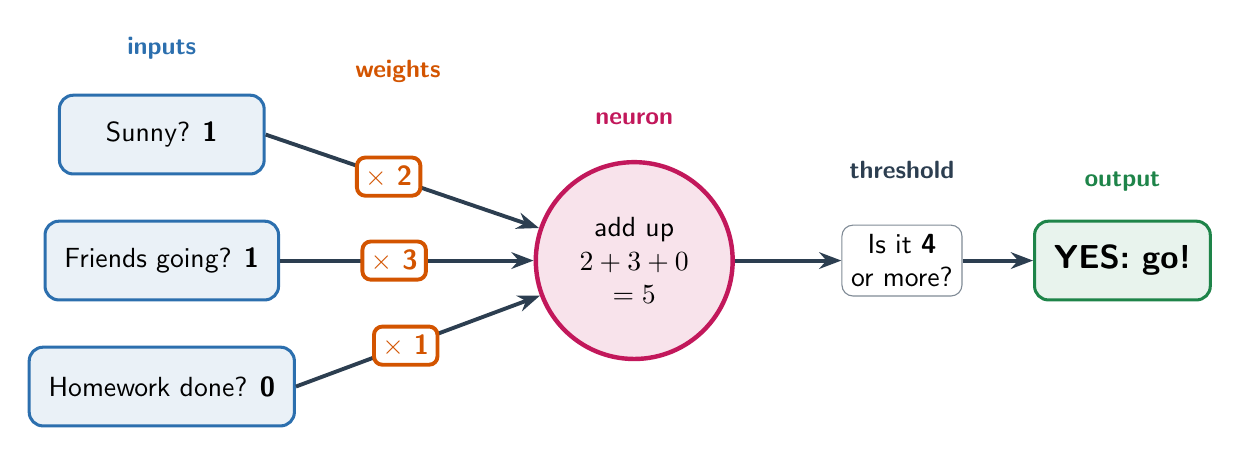
\begin{tikzpicture}[
  inp/.style={personbox, minimum width=2.6cm, font=\normalsize},
  wt/.style={fill=white, draw=machine, rounded corners=3pt, font=\bfseries, text=machine, inner sep=3pt},
]
% An artificial neuron: inputs times weights, add, compare, fire or not.
\node[inp] (i1) at (0,2.2) {Sunny? \textbf{1}};
\node[inp] (i2) at (0,0.6) {Friends going? \textbf{1}};
\node[inp] (i3) at (0,-1.0) {Homework done? \textbf{0}};
\node[draw=brainpink, fill=brainpink!12, circle, line width=1.6pt, minimum size=2.5cm, align=center, font=\normalsize] (n) at (6.0,0.6)
  {add up\\$2 + 3 + 0$\\$= 5$};
\foreach \i/\w in {i1/2, i2/3, i3/1} {
  \draw[flow] (\i.east) -- node[wt, pos=0.45] {$\times$ \w} (n);
}
\node[draw=ink!60, fill=white, rounded corners=4pt, font=\normalsize, align=center] (th) at (9.4,0.6) {Is it \textbf{4}\\or more?};
\draw[flow] (n) -- (th);
\node[resultbox, font=\large\bfseries] (out) at (12.2,0.6) {YES: go!};
\draw[flow] (th) -- (out);
\node[font=\small\bfseries, text=person] at (0,3.3) {inputs};
\node[font=\small\bfseries, text=machine] at (3.0,3.0) {weights};
\node[font=\small\bfseries, text=brainpink] at (6.0,2.4) {neuron};
\node[font=\small\bfseries, text=ink] at (9.4,1.75) {threshold};
\node[font=\small\bfseries, text=result] at (12.2,1.6) {output};
\end{tikzpicture}
\end{document}
